
\documentclass[11pt]{article}


% Use wide margins, but not quite so wide as fullpage.sty
\marginparwidth 0.4in 
\oddsidemargin 0.2in 
\evensidemargin 0.2in 
\marginparsep 0.2in
\topmargin 0.2in 
\textwidth 6in \textheight 8 in
% That's about enough definitions

% multirow allows you to combine rows in columns
\usepackage{multirow}
% tabularx allows manual tweaking of column width
\usepackage{tabularx}
% longtable does better format for tables that span pages
\usepackage{longtable}
\usepackage{graphicx}
\usepackage{amssymb} % needed for math
\usepackage{amsmath} % needed for math
\usepackage{listings} % needed for the inclusion of source code
\usepackage{mips}

\usepackage{color}

\definecolor{dkgreen}{rgb}{0,0.6,0}
\definecolor{gray}{rgb}{0.5,0.5,0.5}
\definecolor{mauve}{rgb}{0.58,0,0.82}

\lstset{ %
  language=[mips]Assembler,       % the language of the code
  basicstyle=\footnotesize,       % the size of the fonts that are used for the code
  numbers=left,                   % where to put the line-numbers
  numberstyle=\tiny\color{gray},  % the style that is used for the line-numbers
  stepnumber=1,                   % the step between two line-numbers. If it's 1, each line 
                                  % will be numbered
  numbersep=5pt,                  % how far the line-numbers are from the code
  backgroundcolor=\color{white},  % choose the background color. You must add \usepackage{color}
  showspaces=false,               % show spaces adding particular underscores
  showstringspaces=false,         % underline spaces within strings
  showtabs=false,                 % show tabs within strings adding particular underscores
  frame=single,                   % adds a frame around the code
  rulecolor=\color{black},        % if not set, the frame-color may be changed on line-breaks within not-black text (e.g. commens (green here))
  tabsize=4,                      % sets default tabsize to 2 spaces
  captionpos=b,                   % sets the caption-position to bottom
  breaklines=true,                % sets automatic line breaking
  breakatwhitespace=false,        % sets if automatic breaks should only happen at whitespace
  title=\lstname,                 % show the filename of files included with \lstinputlisting;
                                  % also try caption instead of title
  keywordstyle=\color{blue},          % keyword style
  commentstyle=\color{dkgreen},       % comment style
  stringstyle=\color{mauve},         % string literal style
  escapeinside={\%*}{*)},            % if you want to add a comment within your code
  morekeywords={*,...}               % if you want to add more keywords to the set
}

% this is needed for forms and links within the text
\usepackage{hyperref}  

\begin{document}
% this is an alternate method of creating a title
%\hfill\vbox{\hbox{Gius, Mark}
%       \hbox{Cpe 456, Section 01}  
%       \hbox{Lab 1}    
%       \hbox{\today}}\par
%
%\bigskip
%\centerline{\Large\bf Lab 1: Security Audit}\par
%\bigskip
\author{Name Surname, Student ID}
\title{BBM234: Computer Organization\\MIPS Project Report}
\maketitle

\section{Problem: Arrays Using for Loops}

MIPS Assembly code:

\begin{lstlisting}
	.data
A: .word 2, 4, 6, 8

	.text
	.globl main
main:
	la $t0, A # load the address of A[0] into $t0
	# The rest of your code...
	# Don't forget to write comments!
done:
	jr $ra # return
\end{lstlisting}

Your explanation, results, screenshots...

Example how to include a screenshot: Fig. \ref{fig:1test1bef}.
    
    
    \begin{figure}[h!]
            \centering
            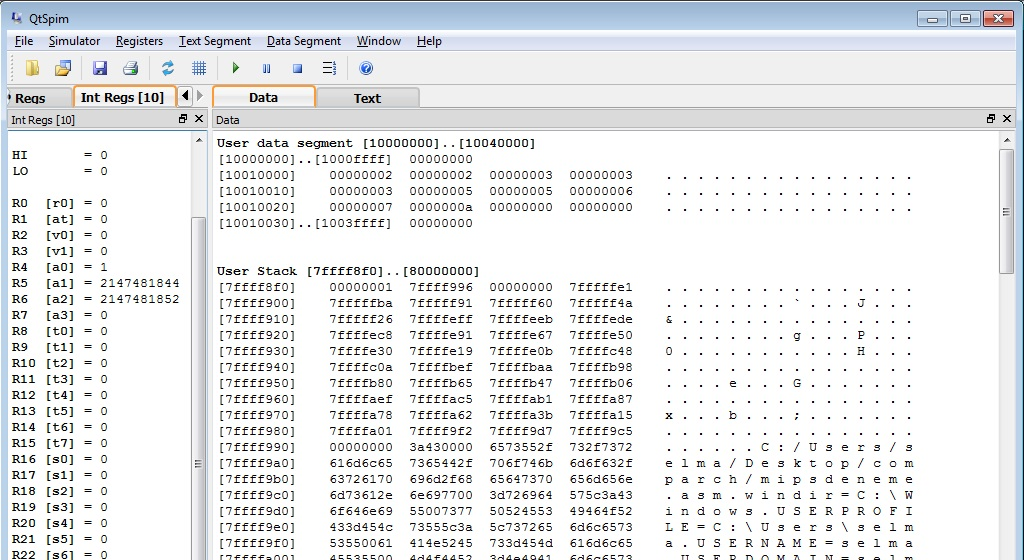
\includegraphics[width=17cm]{screenshot.jpg}
            \caption{Test 1: before}
            \label{fig:1test1bef}
    \end{figure}
        
  
\clearpage
\newpage


\section{Problem: Function Calls}

MIPS Assembly code:
\begin{lstlisting}
	.text
	.globl main
main:
    # Your code...
    # Don't forget to write comments!

\end{lstlisting}

Your explanation, results, screenshots...
\newline

Notes: 
\begin{itemize}
    \item {Note 1...}
    \item {Note 2...}
\end{itemize}


\end{document}
